\documentclass[a4paper,11pt]{article}

\usepackage[utf8]{inputenc}

\usepackage[spanish]{babel}
\usepackage{amsmath}%paquete matemático
\usepackage{amsfonts}% proporciona caracteres para ciertos conjuntos matematicos
\usepackage{eurosym}% paquete para simbolo euro
\usepackage[pdftex]{graphicx}%para insertar figuras .png o .jpg
\usepackage{float}
%\parindent=20px

%\parskip=2cm

\begin{document}
 \listoffigures% indice de imagenes
\part{Matemáticas II}
\section{Tipos de letras matemáticas}
%Usando $formula_matematica$
%Usando begin align,displaymath,equation para activar el mathmode en LATEX
\begin{align}
\mathnormal{Normal}\\
\mathrm{Rematada}
\end{align}
$\mathcal{R\:Z\:Q}$ \\% NECESITA AMSFONTS
$\mathbb{R\:Z\:Q}$ \\% NECESITA AMSFONTS
$\mathfrak{R\:Z\:Q}$ \\ % NECESITA AMSFONTS
\begin{displaymath}
  \mathit{Cursiva}\\
  \mathbf{Negrita} \\
  \end{displaymath}
  \begin{displaymath}
  \mathsf{sans-serif\:font} \\
  \mathtt{De\:maquina} \\
  \mathcal{R\:Z\:Q}
\end{displaymath}

\section{Simbolos encima de otros}
$\overset{OSL}{\Longleftarrow\Longrightarrow}$
$\underset{n}{\sum}$
$\underset{OSL}{\Longleftarrow\Longrightarrow}$
$\xrightarrow[OSL]{LSO}$
$\xleftarrow[OSL]{LSO}$
\section{Enfatizar textos}
\emph{Si queremos enfatizar un fragmento de texto ya enfatizado, entonces \LaTeX\ usa el modo \emph{normal} para enfatizar.}
\section{Uso de llaves}
$ \underbrace {Hola Mundo} $
$ \overbrace {Hola Mundo} $
$\displaystyle \sum$%modo matematico
$\sum$%modo texto
\section{Dejar espacios}
hola%%generando espacios con \hspace{longitud} podemos generar espacios mas largos "longitud tiene valor numerico"
\,hola
\section{Euro}
 solo modo texto no matemático \euro\
 \part{Comandos Propios}
 \newcommand{\nombre}{definicion}
 ejemplo:
 \newcommand{\einstein}{$E=mc^2$}
 \einstein\
\part{Fotos}
\begin{figure}[!h]
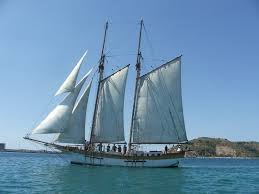
\includegraphics[scale=.75]{indice.jpg} %ruta de la página
\caption{Foto}%% pie de pagina
\label{fig:indice.jpg}
\end{figure}

\end{document}
